\begin{frame}{Aufgabe 3: Basisband II}
  \begin{center}
  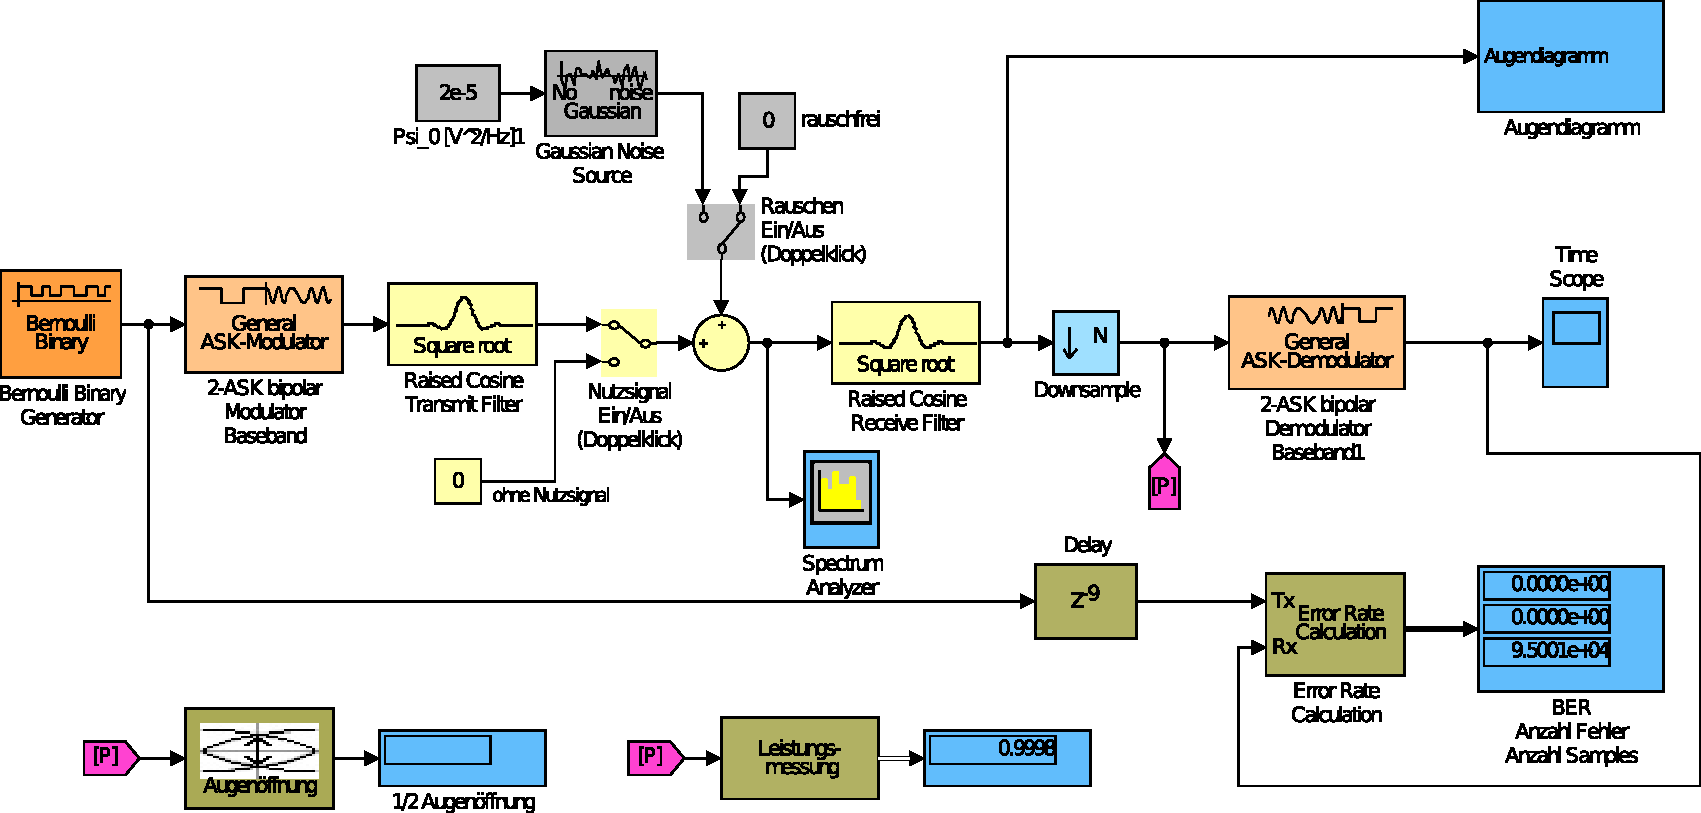
\includegraphics[width=\textwidth]{screenshots/Aufgabe3/modell}
  \end{center}
\end{frame}

\begin{frame}{Aufgabe 3: Basisband II}
  \twocolumns{
    \[B \approx 2.76 \, \si{\kilo\hertz}\]
    }{
      \begin{center}
  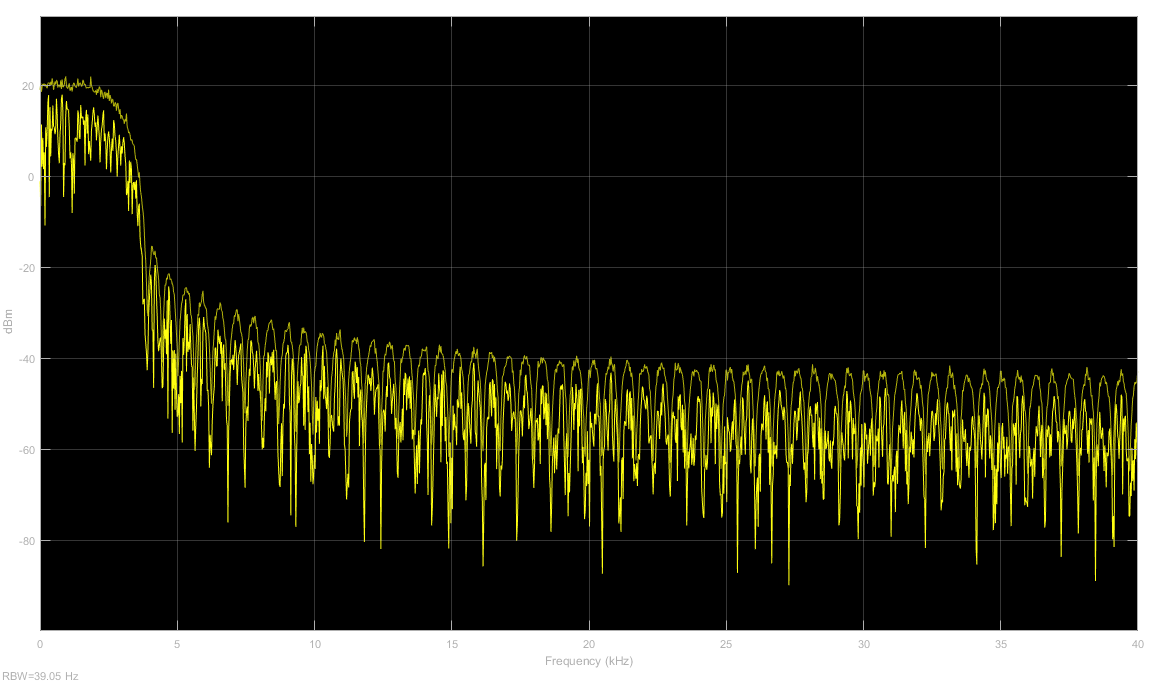
\includegraphics[width=0.854102\textwidth]{screenshots/Aufgabe3/spektrum_sendesignal}
  \end{center}
  }{0.0901699\textwidth}
\end{frame}

\begin{frame}{Aufgabe 3: Basisband II}
  \twocolumns{
    \[U_\mathrm{A} \approx 0.9965 \, \si{\volt}\]
    \[P_\mathrm{R} \approx 0.1 \, \si{\volt}^2\]
    }{
      \begin{center}
  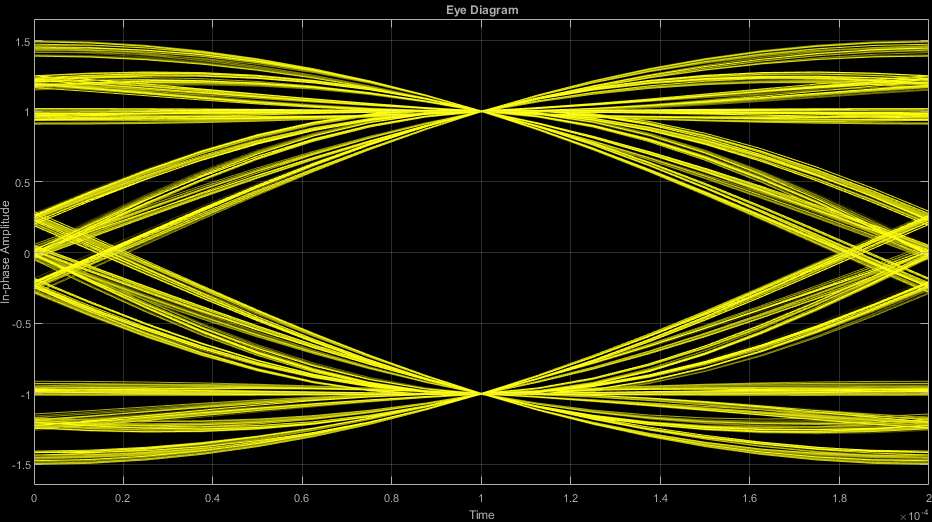
\includegraphics[width=0.854102\textwidth]{screenshots/Aufgabe3/auge_sendesignal}
  \end{center}
  }{0.0901699\textwidth}
\end{frame}

\begin{frame}{Aufgabe 3: Basisband II}
  \[\mathrm{BER} = \frac{1}{\log_2{s}} \cdot \frac{s-1}{s} \cdot
    \mathrm{erfc}{\left(\sqrt{\frac{\rho}{2}}\right)}, \, s = 2\]
  \[\mathrm{BER} = 0.5 \cdot \mathrm{erfc}{\left( \sqrt{\frac{9.93}{2}}
      \right)} = 8.1303 \cdot 10^{-4}\]
  gemessen:
  \[\mathrm{BER}_g = 8.86315 \cdot 10^{-4}\]
\end{frame}